\documentclass{standalone}
\usepackage{tikz}
\usetikzlibrary{patterns, positioning}
\usepackage[sfdefault]{ClearSans} %% option 'sfdefault' activates Clear Sans as the default text font
\usepackage[T1]{fontenc}

\begin{document}
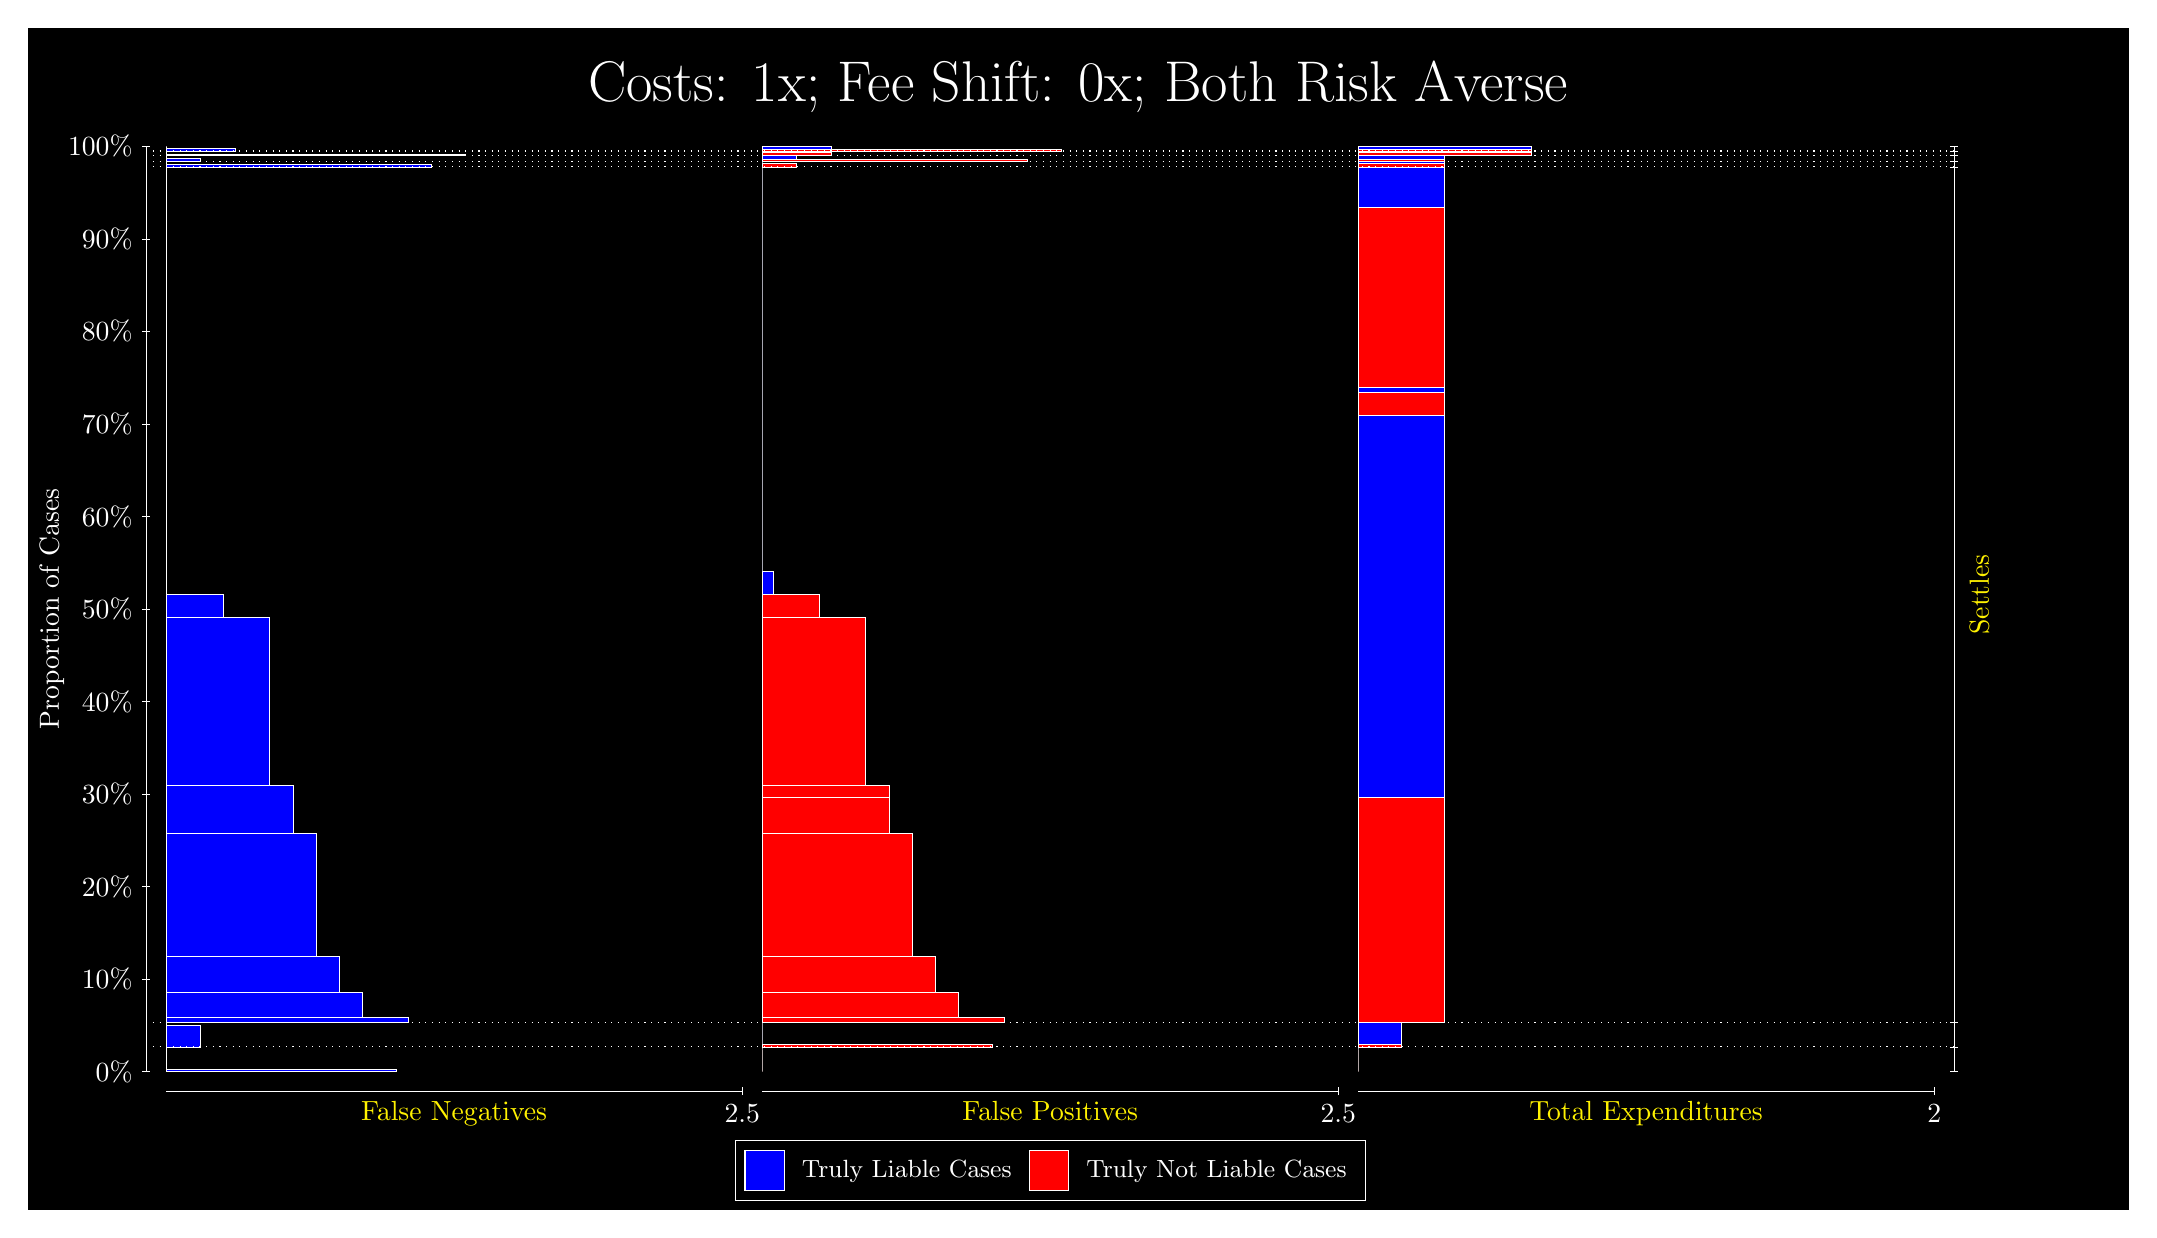
\begin{tikzpicture}
\draw[fill=black] (0,0) rectangle (26.667,15);
\draw[text=white] (0,13.5) rectangle (26.667,15) node[midway] {\huge Costs: 1x; Fee Shift: 0x; Both Risk Averse};
\draw[white, very thin] (1.5,1.75) -- (1.5,13.5);
\node[rotate=90, text=white, anchor=center] at (0.3, 7.625) {Proportion of Cases};
\draw[white, very thin] (1.45,1.75) -- (1.55,1.75);
\node[text=white, anchor=east] at (1.45, 1.75) {0\%};
\draw[white, very thin] (1.45,2.925) -- (1.55,2.925);
\node[text=white, anchor=east] at (1.45, 2.925) {10\%};
\draw[white, very thin] (1.45,4.1) -- (1.55,4.1);
\node[text=white, anchor=east] at (1.45, 4.1) {20\%};
\draw[white, very thin] (1.45,5.275) -- (1.55,5.275);
\node[text=white, anchor=east] at (1.45, 5.275) {30\%};
\draw[white, very thin] (1.45,6.45) -- (1.55,6.45);
\node[text=white, anchor=east] at (1.45, 6.45) {40\%};
\draw[white, very thin] (1.45,7.625) -- (1.55,7.625);
\node[text=white, anchor=east] at (1.45, 7.625) {50\%};
\draw[white, very thin] (1.45,8.8) -- (1.55,8.8);
\node[text=white, anchor=east] at (1.45, 8.8) {60\%};
\draw[white, very thin] (1.45,9.975) -- (1.55,9.975);
\node[text=white, anchor=east] at (1.45, 9.975) {70\%};
\draw[white, very thin] (1.45,11.15) -- (1.55,11.15);
\node[text=white, anchor=east] at (1.45, 11.15) {80\%};
\draw[white, very thin] (1.45,12.325) -- (1.55,12.325);
\node[text=white, anchor=east] at (1.45, 12.325) {90\%};
\draw[white, very thin] (1.45,13.5) -- (1.55,13.5);
\node[text=white, anchor=east] at (1.45, 13.5) {100\%};

\draw[white, very thin] (24.457,1.75) -- (24.457,13.5);
\draw[white, very thin] (24.407,1.75) -- (24.507,1.75);
\node[anchor=west] at (24.407, 1.75) {};
\draw[white, very thin] (24.407,2.0623) -- (24.507,2.0623);
\node[anchor=west] at (24.407, 2.0623) {};
\draw[white, very thin] (24.407,2.3746) -- (24.507,2.3746);
\node[anchor=west] at (24.407, 2.3746) {};
\draw[white, very thin] (24.407,13.239) -- (24.507,13.239);
\node[anchor=west] at (24.407, 13.239) {};
\draw[white, very thin] (24.407,13.31) -- (24.507,13.31);
\node[anchor=west] at (24.407, 13.31) {};
\draw[white, very thin] (24.407,13.382) -- (24.507,13.382);
\node[anchor=west] at (24.407, 13.382) {};
\draw[white, very thin] (24.407,13.441) -- (24.507,13.441);
\node[anchor=west] at (24.407, 13.441) {};
\draw[white, very thin] (24.407,13.5) -- (24.507,13.5);
\node[anchor=west] at (24.407, 13.5) {};

\draw[white, very thin, fill=blue] (1.75,1.75) rectangle (4.6775,1.7829);
\draw[white, very thin, fill=red] (1.75,1.7829) rectangle (1.75,2.0623);
\draw[white, very thin, fill=blue] (1.75,2.0623) rectangle (2.1891,2.3418);
\draw[white, very thin, fill=red] (1.75,2.3418) rectangle (1.75,2.3746);
\draw[white, very thin, fill=blue] (1.75,2.3746) rectangle (4.8239,2.4385);
\draw[white, very thin, fill=blue] (1.75,2.4385) rectangle (4.2384,2.7621);
\draw[white, very thin, fill=blue] (1.75,2.7621) rectangle (3.9457,3.2086);
\draw[white, very thin, fill=blue] (1.75,3.2086) rectangle (3.6529,4.7759);
\draw[white, very thin, fill=blue] (1.75,4.7759) rectangle (3.3602,5.3837);
\draw[white, very thin, fill=blue] (1.75,5.3837) rectangle (3.0674,7.5156);
\draw[white, very thin, fill=blue] (1.75,7.5156) rectangle (2.4819,7.8069);
\draw[white, very thin, fill=red] (1.75,7.8069) rectangle (1.75,13.239);
\draw[white, very thin, fill=blue] (1.75,13.239) rectangle (5.1167,13.269);
\draw[white, very thin, fill=red] (1.75,13.269) rectangle (1.75,13.31);
\draw[white, very thin, fill=blue] (1.75,13.31) rectangle (2.1891,13.351);
\draw[white, very thin, fill=red] (1.75,13.351) rectangle (1.75,13.382);
\draw[white, very thin, fill=blue] (1.75,13.382) rectangle (5.5558,13.402);
\draw[white, very thin, fill=red] (1.75,13.402) rectangle (1.75,13.441);
\draw[white, very thin, fill=blue] (1.75,13.441) rectangle (2.6283,13.48);
\draw[white, very thin, fill=red] (1.75,13.48) rectangle (1.75,13.5);
\draw[white, very thin, fill=red] (9.3189,1.75) rectangle (9.3189,2.0295);
\draw[white, very thin, fill=blue] (9.3189,2.0295) rectangle (9.3189,2.0623);
\draw[white, very thin, fill=red] (9.3189,2.0623) rectangle (12.246,2.0952);
\draw[white, very thin, fill=blue] (9.3189,2.0952) rectangle (9.3189,2.3746);
\draw[white, very thin, fill=red] (9.3189,2.3746) rectangle (12.393,2.4385);
\draw[white, very thin, fill=red] (9.3189,2.4385) rectangle (11.807,2.7621);
\draw[white, very thin, fill=red] (9.3189,2.7621) rectangle (11.515,3.2086);
\draw[white, very thin, fill=red] (9.3189,3.2086) rectangle (11.222,4.776);
\draw[white, very thin, fill=red] (9.3189,4.776) rectangle (10.929,5.2303);
\draw[white, very thin, fill=red] (9.3189,5.2303) rectangle (10.929,5.3837);
\draw[white, very thin, fill=red] (9.3189,5.3837) rectangle (10.636,7.5157);
\draw[white, very thin, fill=red] (9.3189,7.5157) rectangle (10.051,7.807);
\draw[white, very thin, fill=blue] (9.3189,7.807) rectangle (9.4652,8.0982);
\draw[white, very thin, fill=blue] (9.3189,8.0982) rectangle (9.3189,13.239);
\draw[white, very thin, fill=red] (9.3189,13.239) rectangle (9.758,13.28);
\draw[white, very thin, fill=blue] (9.3189,13.28) rectangle (9.3189,13.31);
\draw[white, very thin, fill=red] (9.3189,13.31) rectangle (12.686,13.341);
\draw[white, very thin, fill=blue] (9.3189,13.341) rectangle (9.758,13.382);
\draw[white, very thin, fill=red] (9.3189,13.382) rectangle (10.197,13.42);
\draw[white, very thin, fill=blue] (9.3189,13.42) rectangle (9.3189,13.441);
\draw[white, very thin, fill=red] (9.3189,13.441) rectangle (13.125,13.461);
\draw[white, very thin, fill=blue] (9.3189,13.461) rectangle (10.197,13.5);
\draw[white, very thin, fill=red] (16.888,1.75) rectangle (16.888,2.0295);
\draw[white, very thin, fill=blue] (16.888,2.0295) rectangle (16.888,2.0623);
\draw[white, very thin, fill=red] (16.888,2.0623) rectangle (17.437,2.0952);
\draw[white, very thin, fill=blue] (16.888,2.0952) rectangle (17.437,2.3746);
\draw[white, very thin, fill=red] (16.888,2.3746) rectangle (17.986,5.2303);
\draw[white, very thin, fill=blue] (16.888,5.2303) rectangle (17.986,10.086);
\draw[white, very thin, fill=red] (16.888,10.086) rectangle (17.986,10.377);
\draw[white, very thin, fill=blue] (16.888,10.377) rectangle (17.986,10.441);
\draw[white, very thin, fill=red] (16.888,10.441) rectangle (17.986,12.727);
\draw[white, very thin, fill=blue] (16.888,12.727) rectangle (17.986,13.239);
\draw[white, very thin, fill=red] (16.888,13.239) rectangle (17.986,13.28);
\draw[white, very thin, fill=blue] (16.888,13.28) rectangle (17.986,13.31);
\draw[white, very thin, fill=red] (16.888,13.31) rectangle (17.986,13.341);
\draw[white, very thin, fill=blue] (16.888,13.341) rectangle (17.986,13.382);
\draw[white, very thin, fill=red] (16.888,13.382) rectangle (19.083,13.42);
\draw[white, very thin, fill=blue] (16.888,13.42) rectangle (19.083,13.441);
\draw[white, very thin, fill=red] (16.888,13.441) rectangle (19.083,13.461);
\draw[white, very thin, fill=blue] (16.888,13.461) rectangle (19.083,13.5);
\draw[white, dotted] (1.5,2.0623) -- (24.457,2.0623);
\draw[white, dotted] (1.5,2.3746) -- (24.457,2.3746);
\draw[white, dotted] (1.5,13.239) -- (24.457,13.239);
\draw[white, dotted] (1.5,13.31) -- (24.457,13.31);
\draw[white, dotted] (1.5,13.382) -- (24.457,13.382);
\draw[white, dotted] (1.5,13.441) -- (24.457,13.441);
\draw[white, very thin] (1.75,1.5) -- (9.0689,1.5);
\node[text=yellow, anchor=north] at (5.4094, 1.5) {False Negatives};
\draw[white, very thin] (9.0689,1.45) -- (9.0689,1.55);
\node[text=white, anchor=north] at (9.0689, 1.45) {2.5};

\draw[white, very thin] (9.3189,1.5) -- (16.638,1.5);
\node[text=yellow, anchor=north] at (12.978, 1.5) {False Positives};
\draw[white, very thin] (16.638,1.45) -- (16.638,1.55);
\node[text=white, anchor=north] at (16.638, 1.45) {2.5};

\draw[white, very thin] (16.888,1.5) -- (24.207,1.5);
\node[text=yellow, anchor=north] at (20.547, 1.5) {Total Expenditures};
\draw[white, very thin] (24.207,1.45) -- (24.207,1.55);
\node[text=white, anchor=north] at (24.207, 1.45) {2};



\node[text=yellow, centered, rotate=90] at (24.777, 7.8069) {Settles};





\draw (12.978300999999998,1.5) node[draw=none] (baseCoordinate) {};
\begin{scope}[align=center]
        \matrix[scale=0.5, draw=white, below=0.5cm of baseCoordinate, nodes={draw}, column sep=0.1cm]{
            \node[rectangle, draw, minimum width=0.5cm, minimum height=0.5cm, fill=blue] {}; &
            \node[draw=none, font=\small, text=white] (B) {Truly Liable Cases}; &
            \node[rectangle, draw, minimum width=0.5cm, minimum height=0.5cm, fill=red] {}; &
            \node[draw=none, font=\small, text=white] (B) {Truly Not Liable Cases}; \\
            };
\end{scope}

\end{tikzpicture}
\end{document}